\chapter{Исследовательская часть}

\section{Технические характеристики}

Технические характеристики устройства, на котором выполнялось тестирование:
\begin{itemize}
	\item операционная система: Ubuntu 22.04.1 LTS Linux x86\_64 \cite{ubuntu};
	\item память: 8 ГБ;
	\item процессор: Intel® Core™ i3-7130U.
\end{itemize}

Тестирование проводилось на ноутбуке, включенном в сеть электропитания. Во время тестирования ноутбук был нагружен только встроенными приложениями окружения, окружением, а также непосредственно системой тестирования.

\section{Пример работы программы}

На рисунке \ref{img:example} представлен пример работы программы. Вводятся две строки, в данном случае <<dasha>> и <<arisah>>, размера 5 и 6 соответственно. Для даных строк расстояние Левенштейна равно 5, а расстояние Дамерау -- Левенштейна 4. Это связано с редакторской операцией транспозиции для букв <<a>> и <<h>>. Для итеративных алгоритмов также выводится матрица. Также выводится время выполнения каждого алгоритма в тиках.
\pagebreak 
\begin{figure}[h]
	\centering
	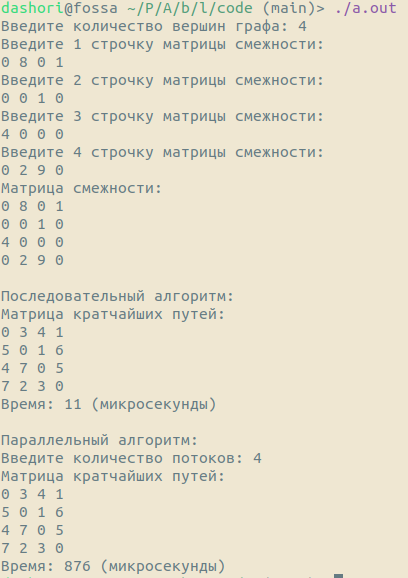
\includegraphics[width=130mm]{example}
	\caption{Пример работы программы}
	\label{img:example}
\end{figure}

\section{Время выполнения реализации алгоритмов}

Время работы реализации алгоритмов было замерено с помощи ассемблерной вставки \ref{lst:time}. Полученное время измеряется в тиках.
\pagebreak
\begin{lstinputlisting}[
	caption={Ассемблерная вставка},
	label={lst:time}
	]{time.cpp}
\end{lstinputlisting}

Замеры времени работы реализованных алгоритмов для определенной длины строк проводились 20 раз, при этом каждый раз строки генерировались случайно. В качестве результата, представленного в таблице \ref{tab:time}, взято среднее время на каждой длине слова. 
\pagebreak
\begin{table}[h]
	\begin{center}
		\caption{\label{tab:time}Результаты замеров времени в тиках}
	\begin{tabular}{|l|l|l|l|l|}
		\hline \specialcell{Длина\\строк} & \specialcell{Итеративный\\(Левенштейн)} &
		 \specialcell{Итеративный} & \specialcell{Рекурсивный \\с кешом} & \specialcell{Рекурсивный} \\\hline
		2   & 5778   & 5507   & 7488    & 5155     \\\hline
		3   & 8599   & 9853   & 13208   & 24538    \\\hline
		4   & 13064  & 20477  & 22773   & 118544   \\\hline
		5   & 14039  & 16225  & 25821   & 385112   \\\hline
		6   & 19453  & 22825  & 32964   & 1623606  \\\hline
		7   & 9429   & 16164  & 13886   & 3112536  \\\hline
		8   & 6611   & 7752   & 11061   & 10516211 \\\hline
		9   & 7515   & 10415  & 17934   & 57280850 \\\hline
		10  & 8042   & 10699  & 14482   & NaN       \\\hline
		11  & 8325   & 10199  & 16205   & NaN        \\\hline
		12  & 9445   & 12121  & 19124   & NaN      \\\hline
		13  & 10948  & 14523  & 21885   & NaN        \\\hline
		14  & 10580  & 17325  & 26895   & NaN        \\\hline
		15  & 13822  & 19294  & 28440   & NaN        \\\hline
		16  & 15863  & 21484  & 32942   & NaN        \\\hline
		17  & 16613  & 23131  & 38527   & NaN        \\\hline
		18  & 19313  & 26357  & 40869   & NaN        \\\hline
		19  & 23353  & 29563  & 45762   & NaN        \\\hline
		20  & 26220  & 35045  & 55871   & NaN        \\\hline
		30  & 49478  & 78967  & 111383  & NaN        \\\hline
		40  & 113762 & 152507 & 246839  & NaN        \\\hline
		50  & 138558 & 193787 & 305259  & NaN        \\\hline
		60  & 193317 & 270063 & 440642  & NaN        \\\hline
		70  & 267411 & 380159 & 668288  & NaN        \\\hline
		80  & 362592 & 499571 & 796852  & NaN        \\\hline
		90  & 566693 & 895042 & 1210304 & NaN      \\\hline
		100 & 585323 & 752124 & 1281518 & NaN		   \\\hline
	\end{tabular}
	\end{center}
\end{table}

На рисунке \ref{img:result4} представлена зависимость времени работы от длины строк итеративных алгоритма поиска расстояния Левенштейна и Дамерау -- Левенштейна, а также рекурсвиного с кешом и без алгоритмов поиска расстояния Дамерау -- Левенштейна. На рисунке \ref{img:result3} представлена зависимость времени работы от длины строк рекурсивного с кешом алгоритма поиска расстояиня Дамерау -- Левенштейна и итеративных алгоритмов поиска расстояния Левенштейна и Дамерау -- Левенштенйна .

\begin{figure}[h]
	\centering
	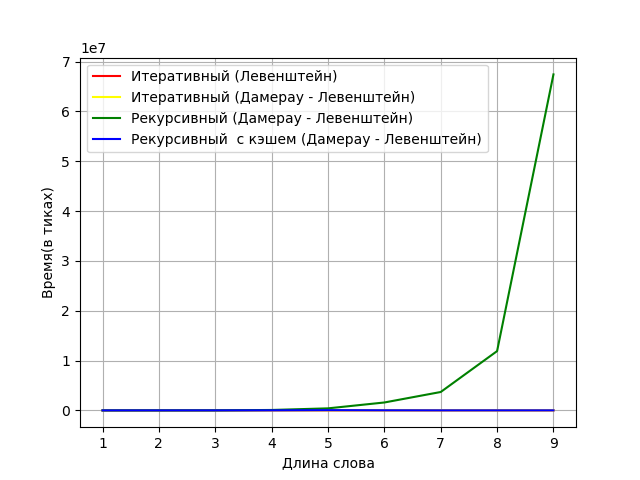
\includegraphics[width=140mm]{result4}
	\caption{Зависимость времени работы от длины строк алгоритмов поиска расстояния Левенштейна и Дамерау -- Левенштейна}
	\label{img:result4}
\end{figure}

\begin{figure}[h]
	\centering
	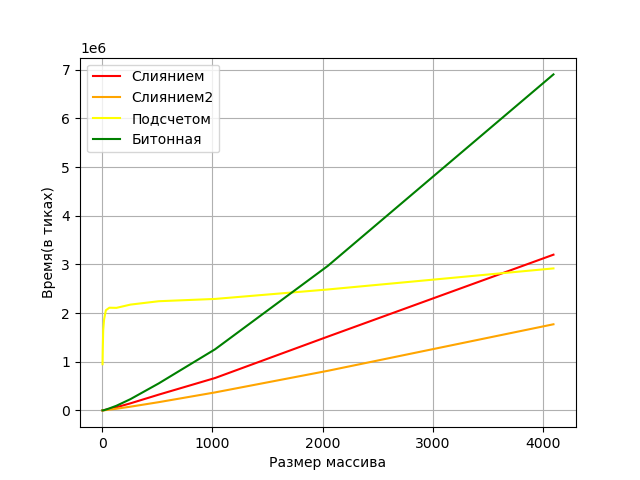
\includegraphics[width=140mm]{result3}
	\caption{Зависимость времени работы от длины строк рекурсивного алгоритма поиска расстояния Дамерау -- Левенштейна и  итеративных алгоритмов поиска расстояния Левенштейна и Дамерау -- Левенштейна}
	\label{img:result3}
\end{figure}


\clearpage
\newpage
\section{Использование памяти}

Рассмотрим разницу рекурсивной и матричной реализаций алгоритмов нахождения расстояния Дамерау -- Левенштейна.

Пусть длина строки $S_{1}$ -- n, длина строки $S_{2}$ - m, тогда затраты памяти на приведенные выше алгоритмы будут следующими:
\begin{itemize}
	\item матричная реализация алгоритма поиска расстояния Левенштейна:\begin{itemize}
		\item строки $S_{1}$, $S_{2}$ -- (m + n) * sizeof(char);
		\item длины строк -- 2 * sizeof(int);
		\item матрица -- ((m + 1) * (n + 1)) * sizeof(int);
		\item текущая строка матрицы -- (n + 1) * sizeof(int);
		\item вспомогательные переменные --  3 * sizeof(int).
	\end{itemize}
\end{itemize}

\begin{itemize}
	\item матричная реализация алгоритма поиска расстояния Дамерау -- Левенштейна:\begin{itemize}
		\item строки $S_{1}$, $S_{2}$ -- (m + n) * sizeof(char);
		\item длины строк -- 2 * sizeof(int);
		\item матрица -- ((m + 1) * (n + 1)) * sizeof(int);
		\item текущая строка матрицы -- (n + 1) * sizeof(int);
		\item вспомогательные переменные --  4 * sizeof(int).
	\end{itemize}
\end{itemize}

Максимальная глубина стека вызовов при рекурсивной реализации равна сумме длин входящий строк.

\begin{itemize}
	\item реализация рекурсивного алгоритма поиска расстояния Дамерау -- Левенштейна с использованием кеша (для каждого вызова):
	\begin{itemize}
		\item строки $S_{1}$, $S_{2}$ -- (m + n) * sizeof(char);
		\item длины строк -- 2 * sizeof(int);
		\item вспомогательные переменные --  2 * sizeof(int);
		\item ссылка на матрицу -- sizeof(int*);
		\item адрес возврата.
	\end{itemize}
	Для всех вызовов еще память для хранения самой матрицы -- ((m + 1) * (n + 1)) * sizeof(int).
	\item реализация рекурсивного алгоритма поиска расстояния Дамерау-Левенштейна(для каждого вызова):\begin{itemize}
		\item строки $S_{1}$, $S_{2}$ -- (m + n) * sizeof(char);
		\item длины строк -- 2 * sizeof(int);
		\item вспомогательная переменная -- sizeof(int);
		\item адрес возврата.
	\end{itemize}
\end{itemize}
